\section[面向字节的IO接口]{面向字节的IO接口}
InputStream和OutputStream是面向字节的IO接口,它们处理的是字节流

\subsection[InputStream]{InputStream}
\begin{figure}
  \centering
  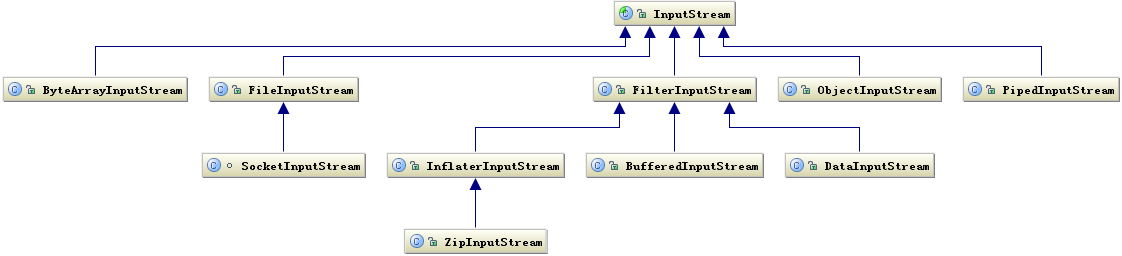
\includegraphics[width=.9\textwidth]{picturedir/inputstream.png}
  \caption{面向字节的InputStream接口}
  \label{fig:inputstream}
\end{figure}

图\ref{fig:inputstream}展示了InputStream的基本接口。
InputStream是一个抽象类,真正使用时都是使用其子类进行实例化。

\subsubsection[FileInputStream]{FileInputStream}
\subsubsection[ByteArrayInputStream]{ByteArrayInputStream}
\subsubsection[ObjectInputStream]{ObjectInputStream}
\subsubsection[PipedInputStream]{PipedInputStream}
\subsubsection[FilterInputStream]{FilterInputStream}

\subsection[OutputStream]{OuttputStream}
\begin{figure}
  \centering
  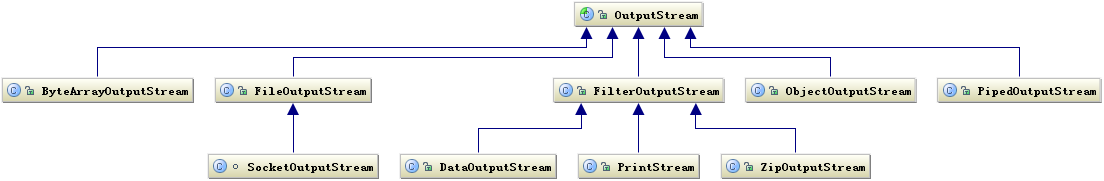
\includegraphics[width=.9\textwidth]{picturedir/outputstream.png}
  \caption{面向字节的OutputStream接口}
  \label{fig:outputstream}
\end{figure}

图\ref{fig:outputstream}展示了OutputStream的基本接口。
OutputStream是一个抽象类,真正使用时都是使用其子类进行实例化。
\subsubsection[FileOutputStream]{FileOutputStream}
\subsubsection[ByteArrayOutputStream]{ByteArrayOutputStream}
\subsubsection[ObjectOutputStream]{ObjectOutputStream}
\subsubsection[PipedOutputStream]{PipedOutputStream}
\subsubsection[FilterOutputStream]{FilterOutputStream}


\section[面向字符的IO接口]{面向字符的IO接口}
\subsection[面向字符的Input接口]{面向字符的Input接口}
\begin{figure}
  \centering
  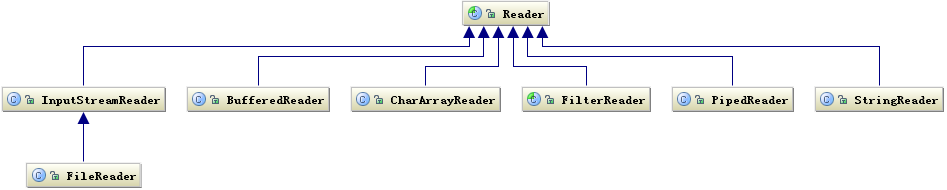
\includegraphics[width=.9\textwidth]{picturedir/reader.png}
  \caption{面向字符的Reader接口}
  \label{fig:reader}
\end{figure}

图\ref{fig:reader}展示了Reader的基本接口。

\subsection[面向字符的Output接口]{面向字符的Output接口}
\begin{figure}
  \centering
  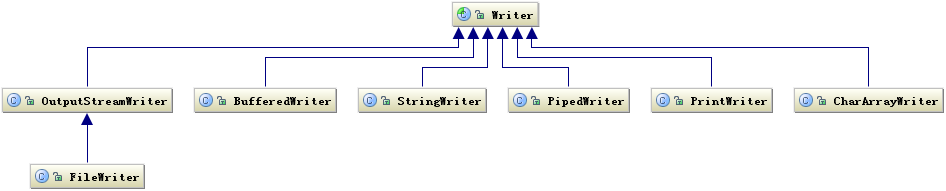
\includegraphics[width=.9\textwidth]{picturedir/writer.png}
  \caption{面向字符的Writer接口}
  \label{fig:writer}
\end{figure}

图\ref{fig:writer}展示了Writer的基本接口。
